\documentclass[a4paper]{article}
\usepackage[utf8]{inputenc}
\usepackage[a4paper, margin=1.5cm, top=1.5cm]{geometry}

\usepackage{graphicx}
\graphicspath{ {images/} }
\usepackage[rightcaption]{sidecap}
\usepackage[margin=1cm]{caption}
\usepackage{subcaption}


\usepackage{amsmath, calc}

\usepackage{verbatim}

\usepackage{listings}
\usepackage{color}

\definecolor{codegreen}{rgb}{0,0.6,0}
\definecolor{codegray}{rgb}{0.5,0.5,0.5}
\definecolor{codepurple}{rgb}{0.58,0,0.82}
\definecolor{backcolour}{rgb}{0.95,0.95,0.92}

\lstdefinestyle{mystyle}{
    backgroundcolor=\color{backcolour},   
    commentstyle=\color{codegreen},
    keywordstyle=\color{magenta},
    numberstyle=\tiny\color{codegray},
    stringstyle=\color{codepurple},
    basicstyle=\footnotesize,
    breakatwhitespace=false,         
    breaklines=true,                 
    captionpos=b,                    
    keepspaces=true,                 
    numbers=left,                    
    numbersep=5pt,                  
    showspaces=false,                
    showstringspaces=false,
    showtabs=false,                  
    tabsize=2
}

\title{Homework - 3}
\author{Sesha Sai Behara}
\begin{document}
\maketitle
\section*{Question 1}
The following are the point group operations which leaves the cluster unchanged:\\
Identity (E) : $\begin{bmatrix} 1 & 0 \\ 0 & 1 \end{bmatrix}$,
Inverse (I) : $\begin{bmatrix} -1 & 0 \\ 0 & -1 \end{bmatrix}$,
Mirror-x (M$_\mathrm{x}$) : $\begin{bmatrix} 1 & 0 \\ 0 & -1 \end{bmatrix}$,
Mirror-y (M$_\mathrm{y}$) : $\begin{bmatrix} -1 & 0 \\ 0 & 1 \end{bmatrix}$.\\
\newline
The force constant matrix can be expressed as a sum over tensor basis:
\begin{equation}
    \begin{bmatrix}
        \phi_{\mathrm{xx}} & \phi_{\mathrm{xy}} \\
        \phi_{\mathrm{yx}} & \phi_{\mathrm{yy}}
    \end{bmatrix} = \phi_{\mathrm{xx}}\begin{bmatrix} 1 & 0 \\ 0 & 0 \end{bmatrix} + \phi_{\mathrm{xy}}\begin{bmatrix} 0 & 1\\ 0 & 0\end{bmatrix} + \phi_{\mathrm{yx}} \begin{bmatrix} 0 & 0 \\ 1 & 0 \end{bmatrix} + \phi_{\mathrm{yy}} \begin{bmatrix} 0 & 0 \\ 0 & 1 \end{bmatrix}      
\end{equation}
To find the symmetry invariant basis, apply Reynold's operator :
\begin{equation}
    \tilde{\Lambda}_{i} =\frac{1}{|\mathrm{S}|}\sum_{\mathrm{S}} \mathrm{S}^{\mathrm{T}} \Lambda_{i}\mathrm{S}
\end{equation}
where $\mathrm{S}$ can be any of the symmetry operator which leaves the cluster unchanged ($\mathrm{E},\mathrm{I},\mathrm{M}_{\mathrm{x}}, \mathrm{M}_{\mathrm{y}}$).\\   
%--------------------------------------------------
Applying Reynold's operator on $\begin{bmatrix} 1 & 0 \\ 0 & 0 \end{bmatrix}$ gives:\\
$    \frac{1}{4} \Bigg(\begin{bmatrix} 1 & 0 \\ 0 & 1 \end{bmatrix} \begin{bmatrix} 1 & 0 \\ 0 & 0\end{bmatrix} \begin{bmatrix} 1 & 0 \\ 0 & 1 \end{bmatrix} + 
\begin{bmatrix} -1 & 0 \\ 0 & -1 \end{bmatrix} \begin{bmatrix} 1 & 0 \\ 0 & 0\end{bmatrix} \begin{bmatrix} -1 & 0 \\ 0 & -1 \end{bmatrix} +  
\begin{bmatrix} 1 & 0 \\ 0 & -1 \end{bmatrix} \begin{bmatrix} 1 & 0 \\ 0 & 0\end{bmatrix} \begin{bmatrix} 1 & 0 \\ 0 & -1 \end{bmatrix} + 
\begin{bmatrix} -1 & 0 \\ 0 & 1 \end{bmatrix} \begin{bmatrix} 1 & 0 \\ 0 & 0\end{bmatrix} \begin{bmatrix} -1 & 0 \\ 0 & 1 \end{bmatrix} \Bigg)$\\
\begin{center} 
$= \frac{1}{4}\begin{bmatrix} 4 & 0 \\ 0 & 0 \end{bmatrix} = \begin{bmatrix} 1 & 0 \\ 0 & 0 \end{bmatrix} $
\end{center}
%---------------------------------------------------
Applying Reynold's operator on $\begin{bmatrix} 0 & 1 \\ 0 & 0 \end{bmatrix}$ gives:\\
$    \frac{1}{4} \Bigg(\begin{bmatrix} 1 & 0 \\ 0 & 1 \end{bmatrix} \begin{bmatrix} 0 & 1 \\ 0 & 0\end{bmatrix} \begin{bmatrix} 1 & 0 \\ 0 & 1 \end{bmatrix} + 
\begin{bmatrix} -1 & 0 \\ 0 & -1 \end{bmatrix} \begin{bmatrix} 0 & 0 \\ 1 & 0\end{bmatrix} \begin{bmatrix} -1 & 0 \\ 0 & -1 \end{bmatrix} +  
\begin{bmatrix} 1 & 0 \\ 0 & -1 \end{bmatrix} \begin{bmatrix} 0 & 1 \\ 0 & 0\end{bmatrix} \begin{bmatrix} 1 & 0 \\ 0 & -1 \end{bmatrix} + 
\begin{bmatrix} -1 & 0 \\ 0 & 1 \end{bmatrix} \begin{bmatrix} 0 & 0 \\ 1 & 0\end{bmatrix} \begin{bmatrix} -1 & 0 \\ 0 & 1 \end{bmatrix} \Bigg)$\\
\begin{center}
$= \frac{1}{4}\begin{bmatrix} 0 & 0 \\ 0 & 0 \end{bmatrix} = \begin{bmatrix} 0 & 0 \\ 0 & 0 \end{bmatrix} $
\end{center}
%----------------------------------------------------
Applying Reynold's operator on $\begin{bmatrix} 0 & 0 \\ 1 & 0 \end{bmatrix}$ gives:\\
$    \frac{1}{4} \Bigg(\begin{bmatrix} 1 & 0 \\ 0 & 1 \end{bmatrix} \begin{bmatrix} 0 & 0 \\ 1 & 0\end{bmatrix} \begin{bmatrix} 1 & 0 \\ 0 & 1 \end{bmatrix} + 
\begin{bmatrix} -1 & 0 \\ 0 & -1 \end{bmatrix} \begin{bmatrix} 0 & 1 \\ 0 & 0\end{bmatrix} \begin{bmatrix} -1 & 0 \\ 0 & -1 \end{bmatrix} +  
\begin{bmatrix} 1 & 0 \\ 0 & -1 \end{bmatrix} \begin{bmatrix} 0 & 0 \\ 1 & 0\end{bmatrix} \begin{bmatrix} 1 & 0 \\ 0 & -1 \end{bmatrix} + 
\begin{bmatrix} -1 & 0 \\ 0 & 1 \end{bmatrix} \begin{bmatrix} 0 & 1 \\ 0 & 0\end{bmatrix} \begin{bmatrix} -1 & 0 \\ 0 & 1 \end{bmatrix} \Bigg)$\\
\begin{center}
$= \frac{1}{4}\begin{bmatrix} 0 & 0 \\ 0 & 0 \end{bmatrix} = \begin{bmatrix} 0 & 0 \\ 0 & 0 \end{bmatrix} $
\end{center}
%--------------------------------------------
Applying Reynold's operator on $\begin{bmatrix} 0 & 0 \\ 0 & 1 \end{bmatrix}$ gives:\\
$    \frac{1}{4} \Bigg(\begin{bmatrix} 1 & 0 \\ 0 & 1 \end{bmatrix} \begin{bmatrix} 0 & 0 \\ 0 & 1\end{bmatrix} \begin{bmatrix} 1 & 0 \\ 0 & 1 \end{bmatrix} + 
\begin{bmatrix} -1 & 0 \\ 0 & -1 \end{bmatrix} \begin{bmatrix} 0 & 0 \\ 0 & 1\end{bmatrix} \begin{bmatrix} -1 & 0 \\ 0 & -1 \end{bmatrix} +  
\begin{bmatrix} 1 & 0 \\ 0 & -1 \end{bmatrix} \begin{bmatrix} 0 & 0 \\ 0 & 1\end{bmatrix} \begin{bmatrix} 1 & 0 \\ 0 & -1 \end{bmatrix} + 
\begin{bmatrix} -1 & 0 \\ 0 & 1 \end{bmatrix} \begin{bmatrix} 0 & 0 \\ 0 & 1\end{bmatrix} \begin{bmatrix} -1 & 0 \\ 0 & 1 \end{bmatrix} \Bigg)$\\
\begin{center}
$= \frac{1}{4}\begin{bmatrix} 0 & 0 \\ 0 & 4 \end{bmatrix} = \begin{bmatrix} 0 & 0 \\ 0 & 1 \end{bmatrix} $
\end{center}
%----------------------------------------
The force constant matrix ($\Phi$) expressed in the symmetry invariant tensor basis is,
\begin{equation}
    \Phi = \alpha_1 \begin{bmatrix} 1 & 0 \\ 0 & 0 \end{bmatrix} + \alpha_2 \begin{bmatrix} 0 & 0 \\ 0 & 1 \end{bmatrix} = \fbox{$\begin{bmatrix} \alpha_1 & 0 \\ 0 & \alpha_2 \end{bmatrix}$} 
\end{equation}
%&= &= &= &= &= &= &= &= &= &= &= &= &= &= &= &= &= 
\section*{Question 2}
Dynamical matrix ($\mathrm{D}$) is given by,
\begin{equation}
    \fbox{$\mathrm{D} = \frac{1}{\mathrm{m}} \sum\limits_{\vec{\mathrm{r}}_l} \Phi(0,\vec{\mathrm{r}}_l) \mathrm{e}^{-\mathrm{i}\vec{\mathrm{k}}.\vec{\mathrm{r}}_l}$}
\end{equation}
where $\vec{\mathrm{r}}_l$ is position vector of the neighboring atoms, $\vec{\mathrm{k}}$ is the crystal momentum and $\Phi$ is the force constant matrix.
To obtain $\mathrm{D}$, we need $\Phi$ of all the nearest neighbors. It can be obtained using the relation: $\Phi(0,\vec{\mathrm{r}}_l) = \mathrm{S}^\mathrm{T}\Phi(0,\vec{\mathrm{r}}_1)\mathrm{S}$, where $\mathrm{S}$ is the symmetry operation which transforms the cluster $(0,\vec{\mathrm{r}}_1)$ to $(0,\vec{\mathrm{r}}_l)$. The following are the force constant matrices for all the 6 pair clusters.\\
\begin{equation*}
    \Phi(0,\mathrm{r}_1) = \begin{bmatrix} \alpha_1 & 0\\ 0 & \alpha_2 \end{bmatrix} 
\end{equation*}

\begin{equation*}
    \Phi(0,\mathrm{r}_2) = \begin{bmatrix} \frac{1}{4}\alpha_1 + \frac{3}{4}\alpha_2 & \frac{\sqrt{3} }{4}(\alpha_1 - \alpha_2) \\ \frac{\sqrt{3} }{4}(\alpha_1 - \alpha_2) & \frac{3}{4}\alpha_1 + \frac{1}{4}\alpha_2   \end{bmatrix} 
\end{equation*}

\begin{equation*}
    \Phi(0,\mathrm{r}_3) = \begin{bmatrix} \frac{1}{4}\alpha_1 + \frac{3}{4}\alpha_2 & \frac{\sqrt{3} }{4}(\alpha_2 - \alpha_1) \\ \frac{\sqrt{3} }{4}(\alpha_2 - \alpha_1) & \frac{3}{4}\alpha_1 + \frac{1}{4}\alpha_2 \end{bmatrix}
\end{equation*}

\begin{equation*}
    \Phi(0,\mathrm{r}_4) = \begin{bmatrix} \alpha_1 & 0 \\ 0 & \alpha_2 \end{bmatrix} 
\end{equation*}

\begin{equation*}
    \Phi(0,\mathrm{r}_5) = \begin{bmatrix} \frac{1}{4}\alpha_1 + \frac{3}{4}\alpha_2 & \frac{\sqrt{3} }{4}(\alpha_1 - \alpha_2) \\ \frac{\sqrt{3} }{4}(\alpha_1 - \alpha_2) & \frac{3}{4}\alpha_1 + \frac{1}{4}\alpha_2 \end{bmatrix} 
\end{equation*}

\begin{equation*}
    \Phi(0, \mathrm{r}_6) = \begin{bmatrix} \frac{1}{4}\alpha_1 + \frac{3}{4}\alpha_2 & \frac{\sqrt{3} }{4}(\alpha_2 - \alpha_1) \\ \frac{\sqrt{3} }{4}(\alpha_2 - \alpha_1) & \frac{3}{4}\alpha_1 + \frac{1}{4}\alpha_2 \end{bmatrix} 
\end{equation*}
Plugging in the force constant matrices in Equation. 4, gives:
\begin{equation}
    \mathrm{D} = \frac{1}{\mathrm{m}} \begin{bmatrix} 2 \alpha_1 \cos(\mathrm{a}\mathrm{k}_\mathrm{x}) + (\alpha_1 + 3\alpha_
2)\cos(\frac{\mathrm{a}}{2}\mathrm{k}_\mathrm{x}) \cos(\frac{\mathrm{a}\sqrt{3}}{2}\mathrm{k}_\mathrm{y}) & -\sqrt{3}(\alpha_1 - \alpha_2) \sin(\frac{\mathrm{a}}{2}\mathrm{k}_\mathrm{x})\sin(\frac{\mathrm{a}\sqrt{3}}{2}\mathrm{k}_\mathrm{y}) \\ -\sqrt{3}(\alpha_1 - \alpha_2) \sin(\frac{\mathrm{a}}{2}\mathrm{k}_\mathrm{x})\sin(\frac{\mathrm{a}\sqrt{3}}{2}\mathrm{k}_\mathrm{y}) & 2\alpha_2\cos(\mathrm{a}\mathrm{k}_\mathrm{x}) + (3\alpha_1+\alpha_2) \cos(\frac{\mathrm{a}}{2}\mathrm{k}_\mathrm{x})\cos(\frac{a\sqrt{3}}{2}\mathrm{k}_\mathrm{y}) \end{bmatrix}   
\end{equation}
\section*{Question 3}
Considering $(\mathrm{a},0)$, $(\frac{a}{2},\frac{a\sqrt{3}}{2})$ to be the real space lattice vectors of the triangular lattice, the reciprocal lattice vectors are given by: $\frac{2\pi}{a}(0,\frac{2}{\sqrt{3}})$ and $\frac{2\pi}{a}(1,\frac{-1}{\sqrt{3}})$.\\
\\
Figure.\ref{fig:1} shows the first Brillouin zone (shaded portion) and some of the high symmetry points (black dots) of the triangular lattice.
\begin{figure}[htpb]
    \centering
    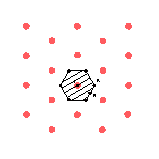
\includegraphics[width=0.7\textwidth]{triangular.pdf}
    \caption{Reciprocal lattice}
    \label{fig:1}
\end{figure}

\section*{Question 4}
The analytical expression for the eigen values of the Dynamical matrix obtained in Question 2 is given by,
\begin{equation}
    \begin{aligned}
    e & = \frac{1}{\mathrm{m}}\Bigg((\alpha_1 + \alpha_2)\Big(\cos(\mathrm{a}\mathrm{k}_\mathrm{x})+2\cos(\frac{\mathrm{a}}{2}\mathrm{k}_\mathrm{x})\cos(\frac{\mathrm{a}\sqrt{3} }{2}\mathrm{k}_\mathrm{y})\Big) \\
    & \pm (\alpha_1 - \alpha_2)\sqrt{\Big(\cos(\mathrm{a}\mathrm{k}_\mathrm{x}) - \cos(\frac{a}{2}\mathrm{k}_\mathrm{x})\cos(\frac{a\sqrt{3}}{2}\mathrm{k}_\mathrm{y})\Big)^2 + 3\sin^2(\frac{a}{2}\mathrm{k}_\mathrm{x})\sin^2(\frac{a\sqrt{3} }{2}\mathrm{k}_\mathrm{y})} \Bigg)
    \end{aligned}
\end{equation}
Figure.\ref{fig:2} shows the dispersion curves along some high symmetry directions ($\Gamma, \mathrm{K}, \mathrm{M}$) for $\mathrm{m}=1$, $\alpha_1=0.1$, and  $\alpha_2=0.2$.
\begin{figure}[htpb]
    \centering
    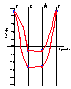
\includegraphics[width=0.6\textwidth]{plot.pdf}
    \caption{Dispersion curves}
    \label{fig:2}
\end{figure}
\section*{Question 5}
The displacement field corresponding to an eigen vector ($\mathrm{e}_{\alpha}$) at a k point ($\vec{\mathrm{k}}$) is given by:  
\begin{equation}
    \vec{\mathrm{u}}({\vec{\mathrm{k}}})= \mathrm{c}\vec{e}_{\alpha}(\vec{\mathrm{k}})
\end{equation}
Figure. \ref{fig:3} shows the displacement field corresponding to the two eigen vectors at $\mathrm{M}$ point. The black and blue arrows represent displacement fields corresponding to 2 different eigen vectors. 
\begin{figure}[htpb]
    \centering
    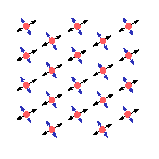
\includegraphics[width=0.6\textwidth]{vec.pdf}
    \caption{Displacement field}
    \label{fig:3}
\end{figure}
\end{document}

